\chapter{Product wise Port Requirements}
\section{Windows Server 2022}
The following are estimated system requirements Windows Server 2022. If computer has less than the minimum requirements, will not be able to install this product correctly. Actual requirements will vary based on system configuration and the applications and features you install.

Processor:
The performance of the processor is determined not only by its clock frequency but also by the number of cores and the size of its cache memory. To ensure smooth operation of Windows Server 2022, the following processor requirements should be met:

Minimum Requirements:
A 64-bit processor with a clock speed of at least 1.4 GHz.
Compatibility with the x64 instruction set.
Support for NX (No-eXecute), which is a security feature that helps prevent malicious code from executing on the processor.
Support for DEP (Data Execution Prevention), another security feature that helps prevent the execution of code in data memory regions.
Support for specific processor instructions including CMPXCHG16b, LAHF/SAHF, and Prefetch, which contribute to improved performance and compatibility with certain software.
Support for Second Level Address Translation (SLAT), also known as Extended Page Tables (EPT) or Nested Page Tables (NPT), a feature that enhances virtualization performance by reducing the overhead of memory address translation.
You can verify whether computer CPU meets these requirements using tools like Core Info.




RAM:
The amount of Random Access Memory (RAM) available in server system significantly impacts its performance, particularly in server environments. Windows Server 2022 has the following RAM requirements:

Minimum Requirements:
512 MB of RAM (2 GB for installations with the Desktop Experience option enabled).
For physical host deployments, Error Correcting Code (ECC) type or similar technology is recommended to ensure data integrity and reliability.
Storage Controller and Disk Space:
Windows Server 2022 requires a storage adapter compliant with the PCI Express architecture specification. Additionally, for servers using hard disk drives, they must not utilize Parallel ATA (PATA). The following are the minimum disk space requirements for the system partition:

Minimum Requirements:
At least 32 GB of disk space is required for the system partition.
Network Adapter:
A reliable network connection is essential for communication and data transfer in server environments. To ensure compatibility and optimal performance, network adapters used with Windows Server 2022 should meet the following requirements:

Minimum Requirements:
An Ethernet adapter capable of throughput of at least gigabit speed (1 Gbps).
Compliance with the PCI Express architecture specification to ensure compatibility with modern server hardware.
By meeting or exceeding these system requirements, you can ensure a stable and efficient installation of Windows Server 2022 on Server hardware configuration. Windows Server 2022 is the latest long-term servicing channel (LTSC) release from Microsoft. It enhances security with secured-core server features and advanced multi-layer protection. The update improves hybrid cloud management and integration with Azure services. It also offers superior application platform capabilities with support for containers. Finally, it provides flexible and scalable storage and compute options for modern workloads.

\newpage

\section{Active Directory Port Requirements}
By Active Directory I meant the Active Directory Domain Services [ADDS]. Below are mentioning the Hardware requirement for ADDS, and the Firewall Ports Requirements.

\begin{figure}[ht]
    \centering
    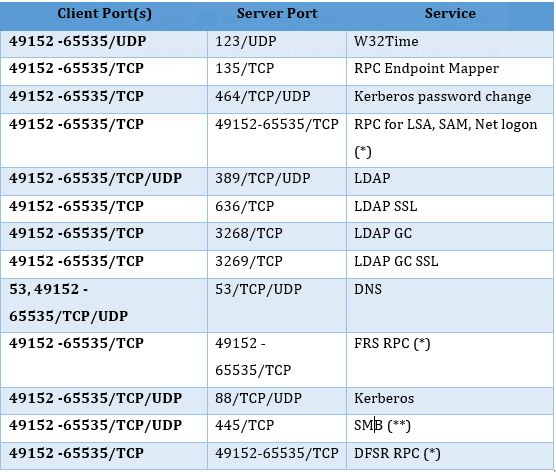
\includegraphics{Chap3/AD.JPG}
    \caption{Active Directory Port Requirements}
    \label{fig:Active Directory Ports}
\end{figure}


\newpage

\section{Mailbox Servers}
Below I mention the Hardware requirement for Mailbox Server, and the Firewall Ports Requirements.
For Mailbox Firewall Port Requirements. Network ports required for clients and services:

\begin{figure}[ht]
    \centering
    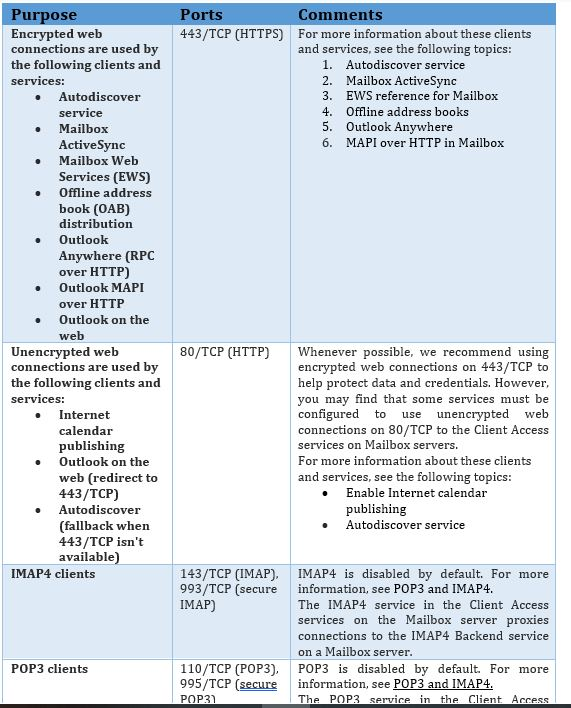
\includegraphics{Chap3/EX01.JPG}
    \caption{Exchange Server port Requirement}
    \label{fig:Exchange Server Ports Requirement}
\end{figure}

\begin{figure}[ht]
    \centering
    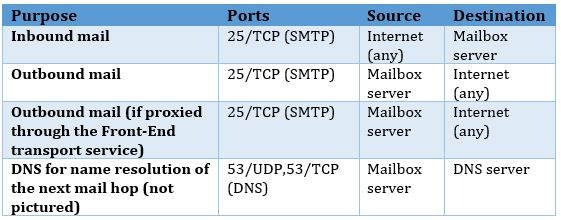
\includegraphics{Chap3/EX02.JPG}
    \caption{Exchange Server port Requirement}
    \label{fig:Exchange Server Ports Requirement}
\end{figure}

\section{Mail Flow with Ports Between Mail Servers}
Below is a revised explanation detailing the TCP ports used by various components of the Mailbox Server transport pipeline, along with the default receive connectors implemented:
Front End Transport Service:
Default Frontend SERVER (TCP 25): This connector handles incoming SMTP connections on port 25.
Outbound Proxy Frontend SERVER (TCP 717): Connections on port 717 are utilized for outbound proxying purposes.
Client Frontend SERVER (TCP 587): This connector manages client submission connections on port 587.


Transport Service:
Default SERVER (TCP 2525): Connections on port 2525 are used for server SMTP connections, which are then proxied to this connector.
Client Proxy SERVER (TCP 465): This connector is responsible for client submission connections on port 465.
Mailbox Transport Service:
SERVER\Default Mailbox Delivery SERVER (TCP 475 - hidden): Cross-server SMTP communication occurs on either TCP 2525 or the hidden port TCP 475.
This revised information provides clarity on the TCP ports utilized by each component, as well as the default receive connectors implemented within the Mailbox Server transport pipeline.
